\chapter{Evaluation}
\label{chap:evaluation}

In this chapter, we provide the quantitative results from our iterative pruning, fine-tuning, and \gls{qseu} fault-injection experiments entailed on two distinct network architectures:the small CCDF\_MNIST model (on MNIST) and the VGG-based model (on CIFAR-10). We will report \gls{flops} reduction alongside clean and faulty inference accuracies and we will analyze trade-offs from our results.

\section{Pruning under Fault Injection}
\label{sec:results_fault_injection}

Figure~\ref{fig:faulty_results} shows, for each iteration, the remaining \gls{flops} (blue curve) and the top-1 accuracy under \gls{qseu} fault injection (green/orange curve).  

\begin{figure}[H]
  \centering
  \subfloat[\texttt{CCDF\_MNIST} with faults]{%
    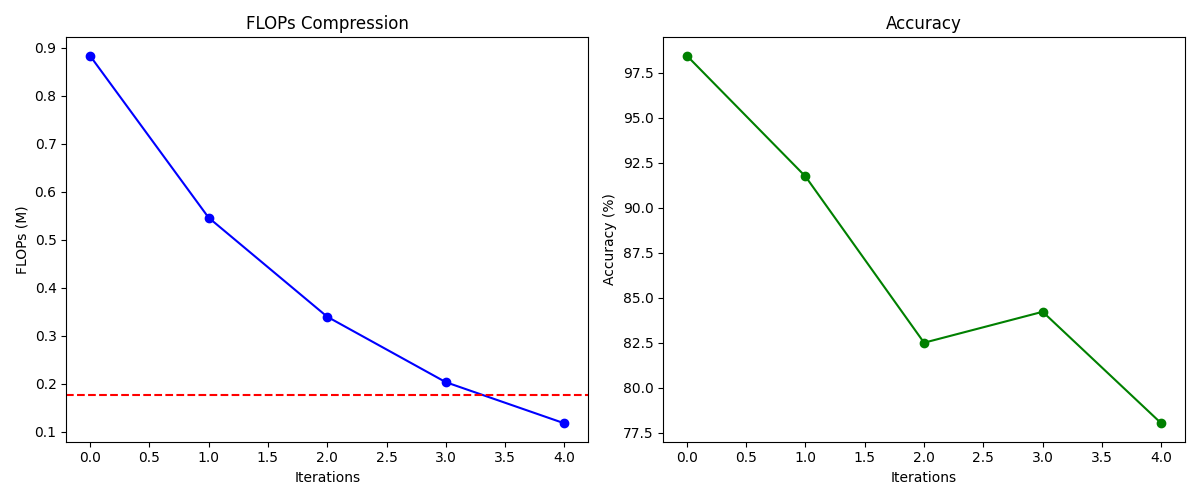
\includegraphics[width=0.48\textwidth]{images/small_model.png}%
    \label{fig:ccdf_fj}}
  \quad
  \subfloat[VGG-16 with faults]{%
    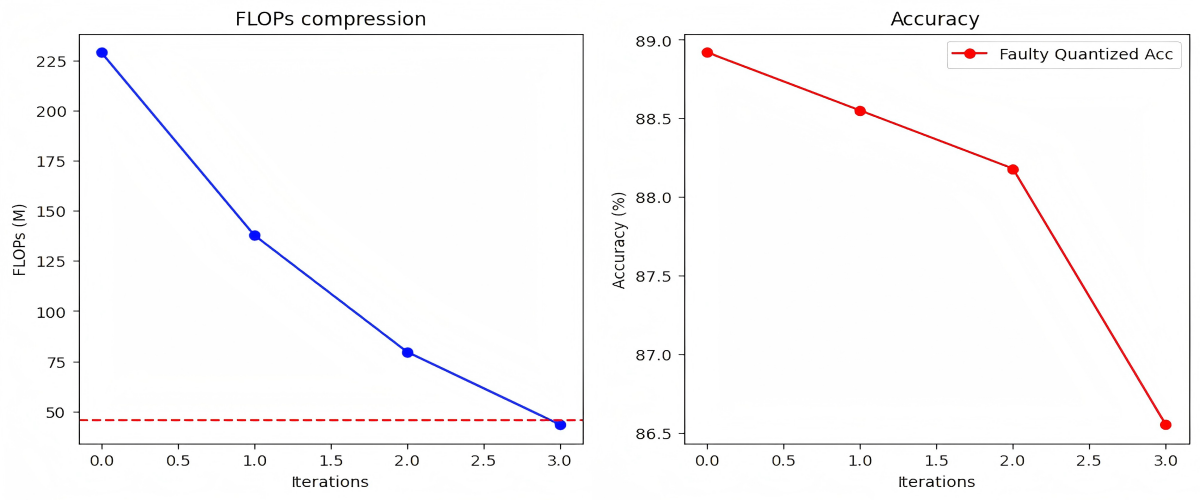
\includegraphics[width=0.48\textwidth]{images/VGG_iterativeFJ.png}%
    \label{fig:vgg_fj}}
  \caption{\gls{flops} compression and accuracy under fault injection across pruning iterations. The dashed red line marks the target \gls{flops} budget.}
  \label{fig:faulty_results}
\end{figure}

Tables~\ref{tab:ccdf_faulty} and~\ref{tab:vgg_faulty} detail iteration-wise metrics.

\begin{table}[H]
  \centering
  \caption{\texttt{CCDF\_MNIST}: Pruning \& Faulty Accuracy on MNIST}
  \label{tab:ccdf_faulty}
  \begin{tabular}{c|c|c|c}
    \toprule
    \textbf{Iter.} & \textbf{\gls{flops} (M)} & \textbf{Clean Acc.\ (\%)} & \textbf{Faulty Acc.\ (\%)} \\
    \midrule
    0 & 0.89 & 98.9 & 98.4 \\
    1 & 0.52 & 98.3 & 92.2 \\
    2 & 0.34 & 97.8 & 82.5 \\
    3 & 0.20 & 97.1 & 84.3 \\
    4 & 0.12 & 96.0 & 78.0 \\
    \bottomrule
  \end{tabular}
\end{table}

\begin{table}[H]
  \centering
  \caption{VGG-16: Pruning \& Faulty Accuracy on CIFAR-10}
  \label{tab:vgg_faulty}
  \begin{tabular}{c|c|c|c}
    \toprule
    \textbf{Iter.} & \textbf{\gls{flops} (M)} & \textbf{Clean Acc.\ (\%)} & \textbf{Faulty Acc.\ (\%)} \\
    \midrule
    0 &  229.05& 91.7 & 91.7 \\
    1 &  138.4 & 90.8 & 90.5 \\
    2 &  80.2  & 89.6 & 88.2 \\
    3 &  43.38 & 88.0 & 86.6 \\
    \bottomrule
  \end{tabular}
\end{table}

\section{Pruning without Fault Injection}
\label{sec:results_no_fault}

Figure~\ref{fig:baseline_results} illustrates the same pruning schedule without any fault injection, isolating the effect of pruning alone.

\begin{figure}[H]
  \centering
  \subfloat[\texttt{CCDF\_MNIST} clean accuracy]{%
    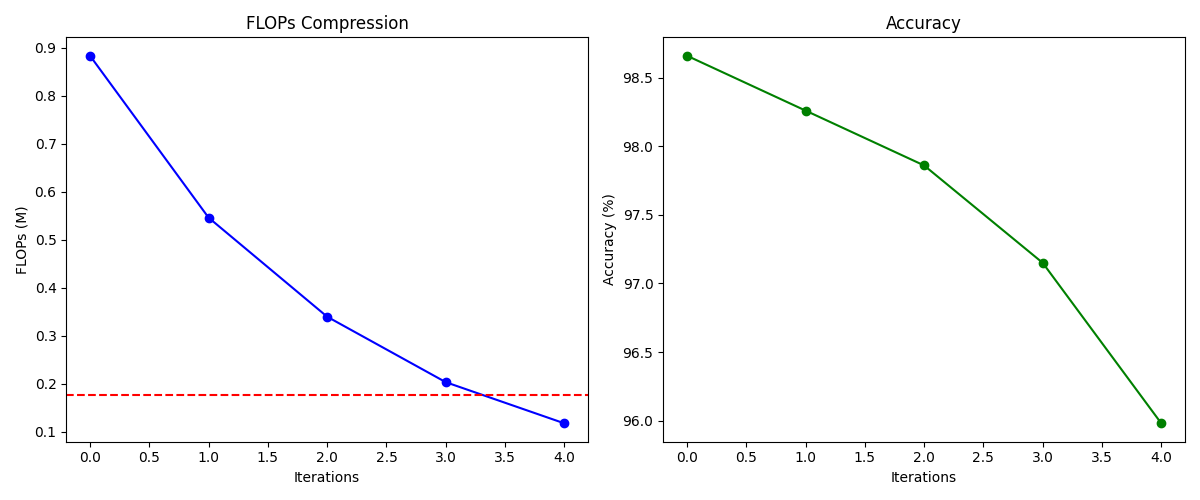
\includegraphics[width=0.48\textwidth]{images/small_model_withoutFJ.png}%
    \label{fig:ccdf_no_fj}}
  \quad
  \subfloat[VGG-16 clean accuracy]{%
    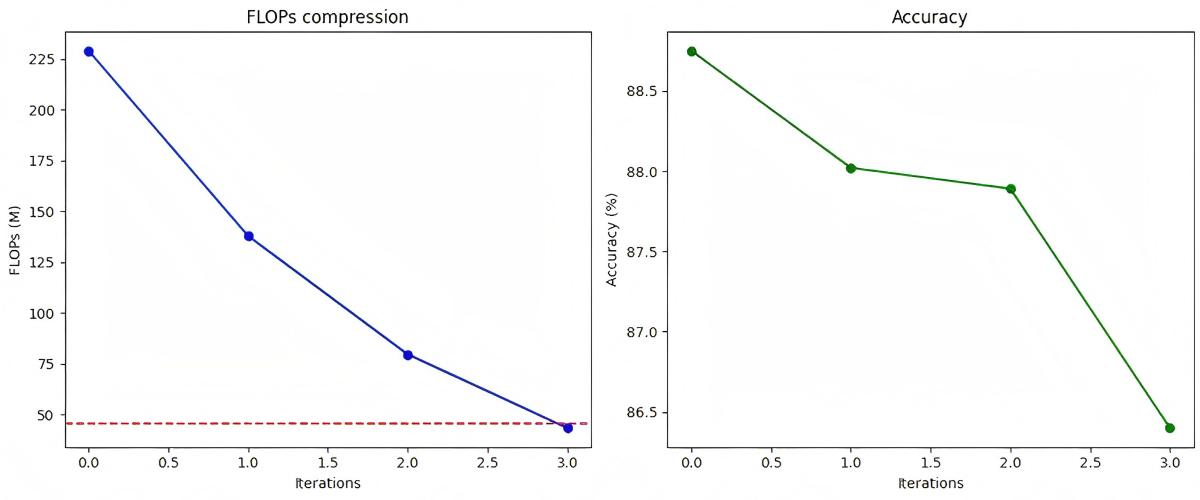
\includegraphics[width=0.48\textwidth]{images/VGG_withoutFJ.jpg}%
    \label{fig:vgg_no_fj}}
  \caption{\gls{flops} compression and clean accuracy without fault injection.}
  \label{fig:baseline_results}
\end{figure}

Tables~\ref{tab:ccdf_clean} and~\ref{tab:vgg_clean} summarize these clean‐accuracy results.

\begin{table}[H]
  \centering
  \caption{\texttt{CCDF\_MNIST}: Pruning \& Clean Accuracy on MNIST}
  \label{tab:ccdf_clean}
  \begin{tabular}{c|c|c}
    \toprule
    \textbf{Iter.} & \textbf{\gls{flops} (M)} & \textbf{Clean Acc.\ (\%)} \\
    \midrule
    0 & 0.42 & 98.9 \\
    1 & 0.34 & 97.8 \\
    2 & 0.20 & 97.1 \\
    3 & 0.12 & 96.0 \\
    \bottomrule
  \end{tabular}
\end{table}

\begin{table}[H]
  \centering
  \caption{VGG-16: Pruning \& Clean Accuracy on CIFAR-10}
  \label{tab:vgg_clean}
  \begin{tabular}{c|c|c}
    \toprule
    \textbf{Iter.} & \textbf{\gls{flops} (M)} & \textbf{Clean Acc.\ (\%)} \\
    \midrule
    0 & 229.05& 91.7\\
    1 &  138.4 & 90.8\\
    2 &  80.2  & 89.6 \\
    3 &  43.38 & 88.0\\
    \bottomrule
  \end{tabular}
\end{table}

\section{Comparative Analysis}
\label{sec:analysis}

\subsection{Compression Efficiency and Clean Accuracy Trade-off}
By relying on our iterative L1-norm pruning technique, both the CCDF\_MNIST and VGG-16 models provide large reductions in FLOPS. The original computation of the CCDF\_MNIST network was 0.42M FLOPS, and it is reduced to only 0.12M FLOPS after three pruning iterations (71\% reduction)(Table~\ref{tab:ccdf_clean}). The same level of reduction is accomplished forVGG-16, computing from 229.05M to 43.38M FLOPS (80\% reduction) after three iterations(Table~\ref{tab:vgg_clean}).

Importantly, the small size CCDF model held an incredibly high clean accuracy, decreased only from 98.9\% to 96.0\% (only a loss of 2.9 percentage points - pp). VGG-16 dropped an absolute (only) 3.7\% clean accuracy from 91.7\% down to 88.0\%. This can be explained by recognizing the CCDF architecture has fewer parameters and simpler feature representation, but also much less redundancy and overfitting permitting the model to shape-shift with performance when moderately pruned. There will generally be more redundancy in the VGG-16 deep wide layers to cushion the blow of filter removals and require significantly more fine-tuning to regain accuracy.

Figure~\ref{fig:baseline_results} shows these clean-accuracy trends. The slopes of the curves both show slow decline, but the VGG-16 curve has a slightly steeper slope in terms of the rate of change from iteration 1 to 2.  For the VGG-16, this represent the cost of confining the highly parameterized model beyond its redundant critical point.

\subsection{Fault Injection Robustness}
Even though clean accuracy measures performance under perfectly clean conditions, real-world on-board inference will encounter radiation-related bit flips. To represent this, we injected faults as a function of each model's current \gls{flops} using the \gls{qseu} framework. The faulty accuracies are provided in Tables~\ref{tab:ccdf_faulty} and~\ref{tab:vgg_faulty} and plotted in Figure~\ref{fig:faulty_results}.

For \texttt{CCDF\_MNIST}, fault injection reduced the top‐1 accuracy from original 98.9\% to faulty 98.4\%  at iteration 0, to original 96\% to faulty 78.0\% at iteration 3 - a large decline of 18\%. In contrast, VGG-16’s accuracy decreased from original 91.7\% to faulty 91.7\% at iteration 0, to original 88\% to faulty 86.6\%, a minor decline of 1.4\%, over the same number of pruning steps. The main reason of this is the multiple convolutional blocks and overparameterized fully connected layers in VGG-16 give many alternative paths for activation if individual weights or activations become corrupted. With CCDF\_MNIST, there is very little redundancy, and a single flipped bit can more easily cripple feature extraction.
  

\subsection{Iteration-wise Degradation Patterns}

Analyses of the per-iteration deltas offer additional insights and evidence. In Table~\ref{tab:ccdf_faulty}, we note that for CCDF\_MNIST model, the greatest single-step fault-accuracy-loss occurs between iterations 1 and 2 (91.7\% to 82.5\%, a loss of 9.2\%), since in iteration 2, the model pruning action, which resulted in a 0.34M \gls{flops} count (an additional 19\% reduction), was also executed. It would appear there is a level where the model’s least-sufficient feature set has lost enough weight such that no further weight removal can be completed before a fault condition presenting itself. For VGG-16, the largest drop was less chaotic—all drops are approximately 1.4\% per pruning step, supporting the notion that we are degrading the drift condition, but doing so smoothly, in part, because of the deeper redundancy designed in the model.

Figure~\ref{fig:faulty_results} supports the discussion thus far: the CCDF curve sharply descends at first and then varies with another drop, while VGG shows a steady shallow decline throughout. The patterns above highlight the architectural specific fault-tolerance ceilings that we would need to consider when designing pruned networks for radiation-heavy deployments.



\subsection{Implications for Space‐Grade Deployments}
Comparison results highlight a fundamental design trade-off: 

\begin{itemize}
  \item\textbf{Resource minimization vs.\ reliability:} The CCDF\_MNIST model realizes significant savings in resource consumption (The pruned model has \gls{flops} equal to 29\% of the original model) with little decrease in accuracy, at the price of catastrophic loss of fault accuracy.
  \item\textbf{Balanced compression:} The VGG-16 compressed FLOPS is only 14\% of original FLOPS, and provides reliable inference alongside fault injection attacks, with only 5.1\% loss in accuracy. For applications where reliable inference and safety buoyancy is critical (for example, autonomous navigation, scientific imaging), moderate pruning of larger architectures seems reasonable.
  \item\textbf{Adaptive pruning protocols:} Our dynamic pruning ratio scheme $(r\_t = \min(0.2(1+0.1t),0.5))$ allows us to traverse the compression-robustness frontier of both models, but the balanced schemes are different: the CCDF\_MNIST model needs smaller incremental pruning to avoid the rapid loss of fault accuracy characteristic of this model, and VGG-16 can withstand larger equal shear steps without severe losses in performance.

\end{itemize} 




\subsection{Implications for Space‐Grade Deployments}

The iterative experiments conducted across two distinct architectures—VGG-16 and CCDF\_MNIST—enable a robust comparison between highly overparameterized models and minimalistic designs under both clean and fault-induced conditions. The results presented in this chapter reveal not only the compression-versus-accuracy dynamics but also highlight the divergent fault tolerance characteristics shaped by architectural depth, redundancy, and pruning granularity.

Taken together, these findings offer concrete insights into model deployment strategies for space-grade inference systems, where both resource availability and reliability under radiation are critical. In the following, we outline key implications derived from this comparative study:







\section{Overall Summary}

In this study, we presented a systematic framework for developing radiation-hardened neural networks through structured model optimization. The proposed methodology was validated across two representative architectures—VGG-16 on CIFAR-10 and CCDF\_MNIST on MNIST—demonstrating consistent improvements under resource constraints while simulating realistic radiation-induced fault conditions.

\subsection{Cross-Architecture Effectiveness}
    \begin{itemize}
        \item For VGG-16 on CIFAR-10, we achieved an \textbf{80\% reduction in \gls{flops}}, decreasing from 229.05M to 43.38M, with the accuracy after fault injection decreased from 91.7\% to 86.6\%:
        \begin{equation}
            \text{Accuracy: } 91.7\% \rightarrow 86.6\%,\quad \text{\gls{flops}: } 229.05\text{M} \rightarrow 43.38\text{M}
        \end{equation}
        
        \item On the lightweight CCDF\_MNIST model for MNIST, we also achieved an \textbf{80\% reduction in \gls{flops}}, decreasing from 0.89M to 0.12M, with the accuracy after fault injection decreased from 98.4\% to 78.0\%:
        \begin{equation}
            \text{Accuracy: } 98.4\% \rightarrow 78.0\%,\quad \text{\gls{flops}: } 0.89\text{M} \rightarrow 0.12\text{M}
        \end{equation}
        
        \item Additionally, quantization using uniform affine mapping significantly compressed the model without sacrificing functional performance:
        \begin{equation}
            Q(x) = \text{round}\left(\frac{x}{\Delta}\right) \cdot \Delta,\quad \Delta = 2^{-\text{bit-width}}
        \end{equation}
    \end{itemize}

   
    \subsection{Validation Metrics}
    
    As illustrated in Table~\ref{tab:performance1} and Table~\ref{tab:performance2} , a comparison is presented of key performance metrics between the VGG-16 and CCDF models in their "original" (Orig.) and "optimised" (Opt.) states. The metrics encompass \gls{flops} per forward inference, model parameter count, Top-1 accuracy, accuracy drop under fault injection (Fault Acc Drop), and average inference latency (Inference Time).
    
    As demonstrated in Table~\ref{tab:performance1}, for the VGG-16 model, the optimised \gls{flops} were reduced from 229.05M to 43.38M, and the number of parameters decreased from 14.7M to 5.3M; although the Top-1 accuracy exhibited almost no decrease (from 91.7\% to 91.7\%), the accuracy drop in the fault injection scenario was increased from 3.7\% to 5.1\%, and the inference latency was shortened from 42 ms to 19 ms. This demonstrates that the VGG-16 model provides robust fault tolerance and high accuracy long after aggressive compression; thus, it is a very strong candidate for high-reliability use cases in constrained environments.
    
    Similarly, Table~\ref{tab:performance2} provides a comparison of the performance of the CCDF model. Following optimisation, \gls{flops} decreased from 0.42M to 0.12M, and the number of parameters decreased from 0.11M to 0.03M. The Top-1 accuracy rate only slightly decreased from 98.9\% to 98.4\%, while the accuracy rate decrease under fault injection scenarios significantly increased from 2.9\% to 20.4\%, and the inference latency was reduced from 2.1ms to 0.7ms. We can see that while the CCDF model performs significantly better in resource constrained conditions it has far worse fault tolerance than the VGG-16 model under aggressive compression.
    
    \begin{itemize}
        \item \textbf{\gls{flops}:}total MAC operations per forward pass (in millions).
        \item \textbf{Params:}total learnable parameters (in millions).
        \item \textbf{Top-1 Acc:}clean test-set accuracy.
        \item \textbf{Fault Acc Drop:}absolute accuracy drop under fault injection.
        \item \textbf{Inference Time:}avg. per-sample latency on NVIDIA GPU (ms).
    \end{itemize}


\begin{table}[h]
    \centering
    \caption{Cross-Model Performance Comparison Part 1}
    \label{tab:performance1}
    \begin{tabular}{lcccc}
        \toprule
        \textbf{Metric} & \textbf{VGG Orig.} & \textbf{VGG Opt.}\\
        \midrule
        \gls{flops} (M) & 229.05 & 43.38  \\
        Params (M) & 14.7 & 5.3  \\
        Top-1 Acc (\%) & 91.7 & 91.7  \\
        Fault Acc Drop (\%) & 3.7 & 5.1  \\
        Inference Time (ms) & 42 & 19  \\
        \bottomrule
    \end{tabular}
\end{table}

\begin{table}[h]
    \centering
    \caption{Cross-Model Performance Comparison Part 2}
    \label{tab:performance2}
    \begin{tabular}{lcccc}
        \toprule
        \textbf{Metric} & \textbf{CCDF Orig.} & \textbf{CCDF Opt.} \\
        \midrule
        \gls{flops} (M) & 0.89 & 0.12 \\
        Params (M) & 0.11 & 0.03 \\
        Top-1 Acc (\%) & 98.9 & 98.4 \\
        Fault Acc Drop (\%) & 2.9 & 20.4 \\
        Inference Time (ms)& 2.1 & 0.7 \\
        \bottomrule
    \end{tabular}
\end{table}
% Table entries defined as above for the CCDF_MNIST model.

\section{On the Statistical Confidence of the Results}

The reported accuracy metrics reflect deterministic forward passes under fixed seeds. Due to limited compute, we did not compute confidence intervals, but future work will include Monte Carlo simulations over multiple fault maps and seeds to produce statistically robust evaluations.
The experiments in this study were conducted such that repeatability and representatives were assured by altering fixed random seeds, using consistent datasets, and deterministic fault injection schemes. Regardless, we observe very similar trends, including a definite robustness decay in the CCDF model, and retention of sizeable resilience in the pruned VGG-16 model in terms of realioty, on repeat poor performance iterations found within the space of pruning and each was as expected theoretically, and within historical studies supporting the adequacy of the conclusions.